\section{Results}
\label{Results}
%\section{Data Analysis}
%\label{Data Analysis}

\subsection{Vertical Radiation Profile}
\begin{figure}[H]
\centering
\begin{subfigure}{.5\textwidth}
  \centering
  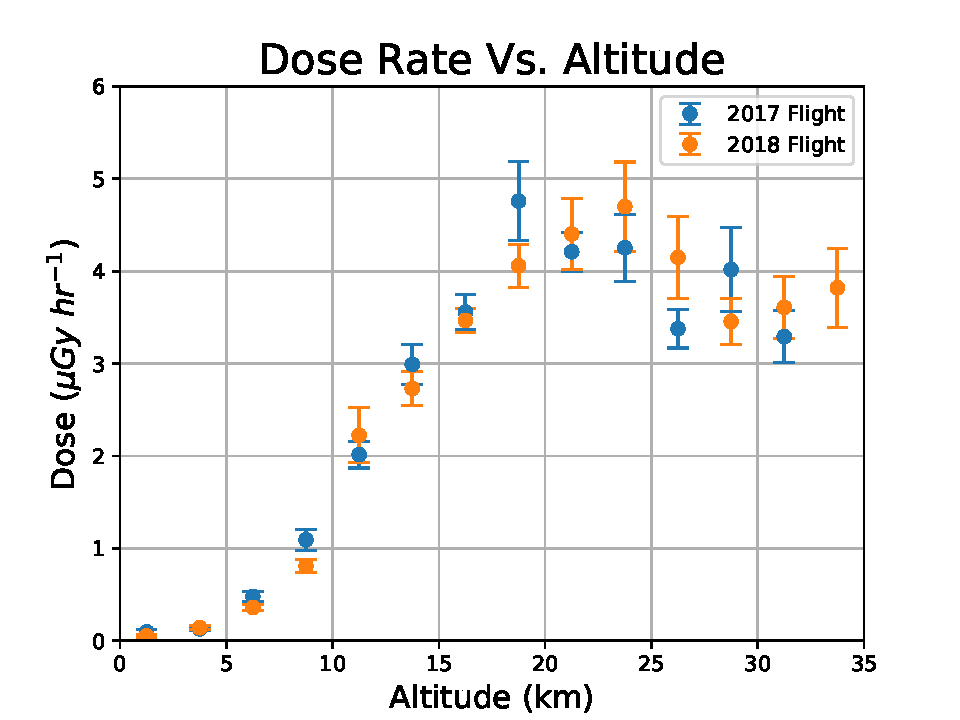
\includegraphics[scale=.45]{dva_stderr.pdf}
  \caption{Dose rate in silicon vs. altitude.}
  \label{fig:sub1}
\end{subfigure}%
\begin{subfigure}{.5\textwidth}
  \centering
  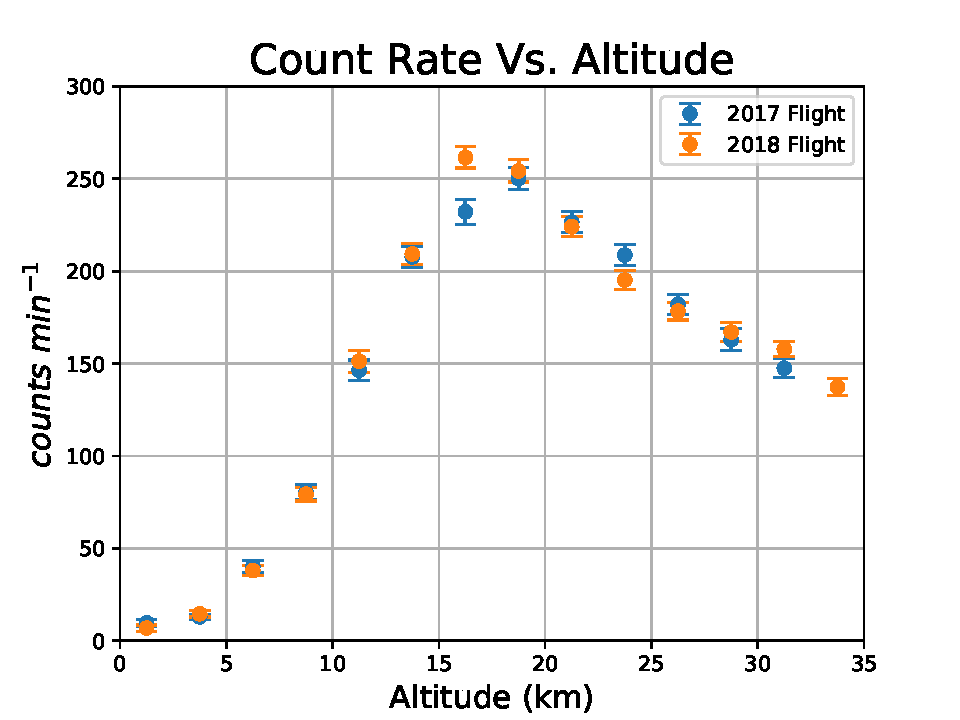
\includegraphics[scale=.45]{cva_stderr.pdf}
  \caption{Detector Hits vs. altitude.}
  \label{fig:sub2}
\end{subfigure}
\caption{Figure ~\ref{fig:sub1} shows the absorbed dose rate per hour as a function of altitude from the MiniPIX.  Figure ~\ref{fig:sub2} shows the counts per minute as a function of altitude again from the MiniPIX data.}
\label{fig:test}
\end{figure}

\begin{figure}[H]
\centering
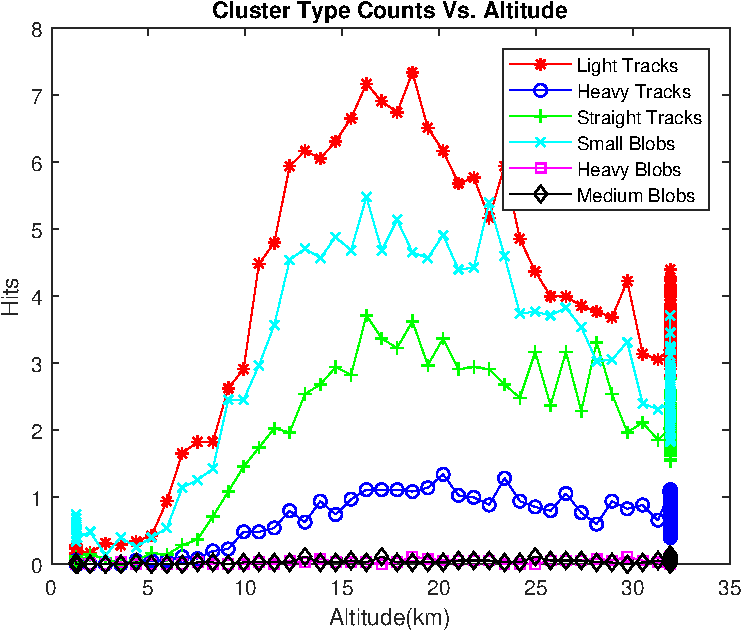
\includegraphics[scale=.5]{ctva-cropped.pdf}
\caption{Cluster Type Counts vs. altitude.}
\end{figure}

\begin{figure}[H]
\centering
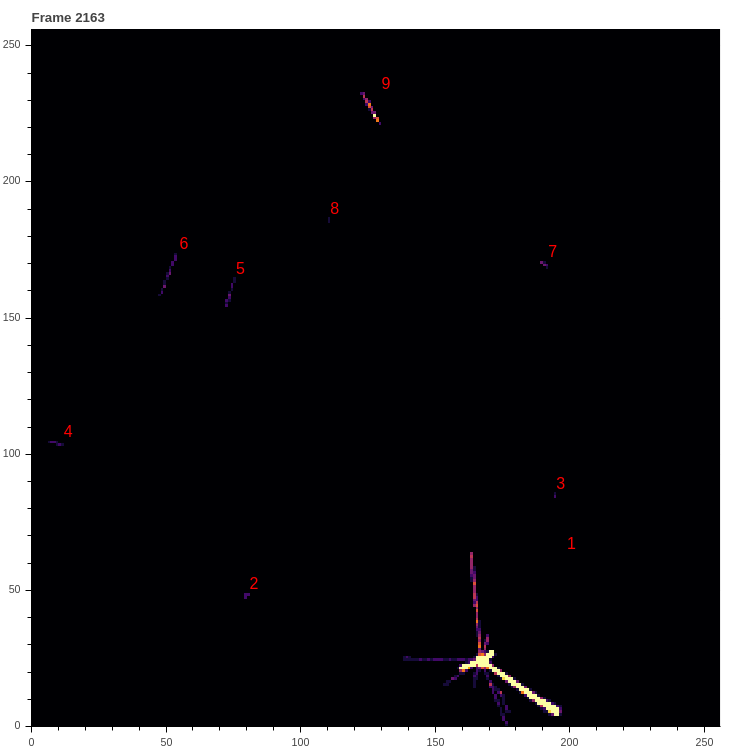
\includegraphics[scale=.35]{tracks.png}
\caption{Frame collected at float.}
\end{figure}
